\documentclass[]{assignment}

\begin{document}


%%% INPUT YOUR NAME AND STUDENT NUMBER
%%% INPUT YOUR NAME AND STUDENT NUMBER
%%% -->
\def\studentname{James Dorrian}
\def\ucdstudentnumber{13369451}
%%% <--
%%% INPUT YOUR NAME AND STUDENT NUMBER
%%% INPUT YOUR NAME AND STUDENT NUMBER


%% HOW TO USE THIS TEMPLATE:
%% No need to keep instruction's text, use this as an template example
%% Replace section content below with your solution
%% Insert Matlab code segments as appropriate
%% Comment and interpret your results 

%% WHAT TO SUBMIT 
%%	1) your pdf report using this latex report
%%	2) an archive of your latex folder
%%  3) your matlab solution in a form of a single commented file


\maketitle


%%%%%%%%%%%%%%%%%%%%%%
%%% 3rd Section

\newpage
\section{{\bf Third Assignment:} Non-side-informed Methods}

In class,  we studied non-side-informed data hiding methods which represent the method that did not exploit a priori knowledge about of the host signal pdf.

%%% First Sub-Section

\subsection{DSSS with known spreading sequence}

The first step was to solve the equation for HWR given by $\mathrm{HWR (dB)}=10\log_{10}{\sigma_X^2}/{D_E},$. I decided to do this using a value of 10 for sigma of X, due to the fact that it solved as an integer value (which equates to 1). After using this result to calculate gamma the next step was to generate a host signal using the values calculated above and attack signal given by $\mathrm{WNR (dB)}=10\log_{10} {D_E}/{\sigma_Z^2}$.

%%% screenshot 1
\begin{figure}[h] 
\centering
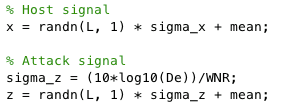
\includegraphics[scale=0.75]{code_snippet1}
\end{figure}

After generating the uniform binary symbol $b$ and pseudorandom vector s, I obtained the watermarked vector by adding the vector generated by the equation $w[i]=b\cdot s[i]\cdot  \gamma$ for all $i=1,\cdots,L$ to the host signal. The attacked watermark vector was then obtained by adding the attack signal to the previously obtained watermarked vector. Finally, I created a function to apply the ML decoder in order to retreive $\hat{b}$ from attacked watermark vector.

%%% screenshot 2
\begin{figure}[h] 
\centering
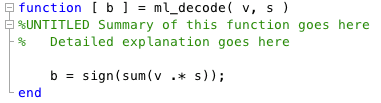
\includegraphics[scale=0.75]{code_snippet2}
\end{figure}

Once $\hat{b}$ was obtained from the attacked watermark vector it is compared to the binary symbol $b$ and if they are NOT equal the decoding error count $c$ was incremented. An empirical probability of decoding error was then calculated by dividing the count by $N$. 

The graphs I obtained for repitiion values of 10,20 and 30 are shown below.

\begin{figure}[h]
\centering
\fboxsep 0mm
\parbox{5cm}{\framebox{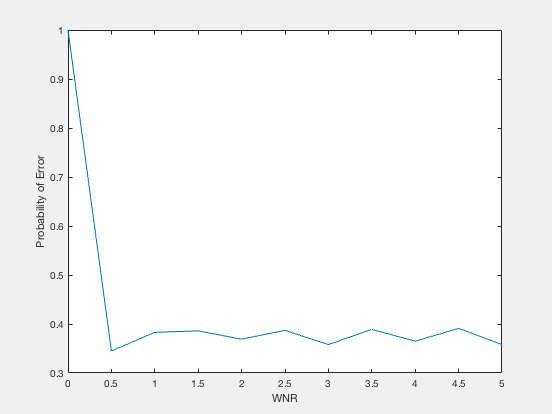
\includegraphics[width=5cm]{L_10}}\\\centering{(a)}}
~~~
\parbox{5cm}{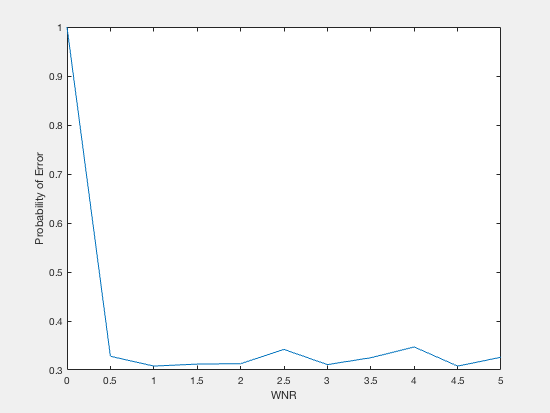
\includegraphics[width=5.05cm]{L_20}\\\centering{(b)}}
~~~
\parbox{5cm}{\framebox{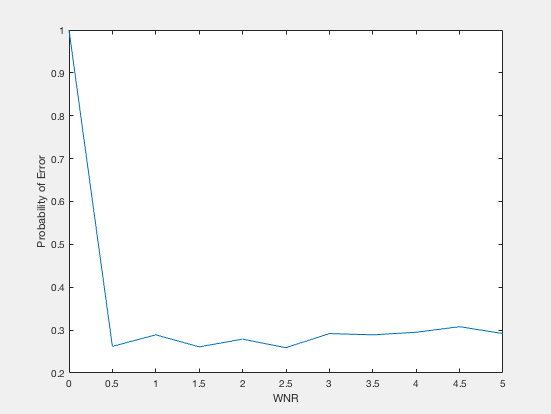
\includegraphics[width=5cm]{L_30}}\\\centering{(c)}}
\caption{\label{fig:imgfilter1} Graphs of P(Detection of Error) vs. WNR where N = 1000}
\end{figure} 

It is clear from these graphs that the probability of the detection of error decreases as the repetition factor increases. The reason for the initial probability of one is that there is no watermark present. (sidenote: although it i hard to see in the document but the minimum value for graph A is $0.35$, for graph B is $0.32$ and for graph C is $0.25$)


%%% Second Sub-Section

\subsection{DSSS with unknown spreading sequence}

Instead of using the pseudorandom vector s mentioned in part 1 we use a new pseudorandom vector in the decoder which implements an unknown spreading sequence. 

Here N = 1000 as outlined in the assignment brief and I used 10 for a value of N. This is the same value of N as used in $fig. 1(a)$. As the below figure clearly illustrates the decoding error is distributed around 0.5 this is the approximate value given to random chance. This is because the decoding is done using a pseudorandom vector which does NOT use the secret key which was used in part 1.

\begin{figure}[h] 
\centering
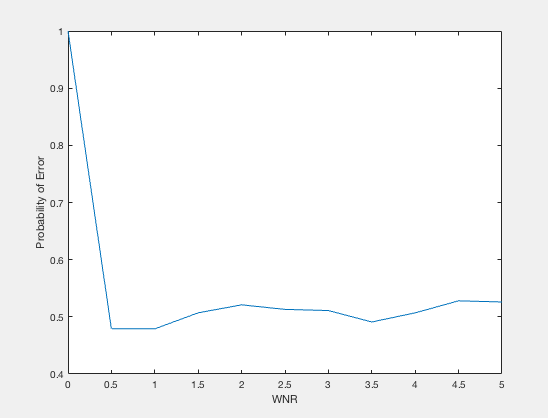
\includegraphics[scale=0.75]{unknown_ss}
\caption{\label{fig:imgfilter1} Decoding without secret key with values of L=10 and N=1000}
\end{figure} 

\label{last_page}

%%%%%%%%%%%%%%%%%%%%%%%%%%%%%%%%%%%
%%%%%%%%%%%%%% END %%%%%%%%%%%%%%%%%%
%%%%%%%%%%%%%%%%%%%%%%%%%%%%%%%%%%%


 \end{document} 